\documentclass[a4paper]{article}

\usepackage[english]{babel}
\usepackage[utf8]{inputenc}
\usepackage{amsmath,amssymb,amsthm}
\usepackage[super]{nth}
\usepackage{listings}
\lstset{
      backgroundcolor=\color{white},   % choose the background color; you must add \usepackage{color} or \usepackage{xcolor}; should come as last argument
      basicstyle=\footnotesize,        % the size of the fonts that are used for the code
      breakatwhitespace=false,         % sets if automatic breaks should only happen at whitespace
      breaklines=true,                 % sets automatic line breaking
      captionpos=b,                    % sets the caption-position to bottom
      commentstyle=\color{green},    % comment style
      deletekeywords={...},            % if you want to delete keywords from the given language
      escapeinside={\%*}{*)},          % if you want to add LaTeX within your code
      extendedchars=true,              % lets you use non-ASCII characters; for 8-bits encodings only, does not work with UTF-8
      frame=single,	                   % adds a frame around the code
      keepspaces=true,                 % keeps spaces in text, useful for keeping indentation of code (possibly needs columns=flexible)
      keywordstyle=\color{blue},       % keyword style
      language=matlab,                 % the language of the code
      morekeywords={*,...},            % if you want to add more keywords to the set
      numbers=left,                    % where to put the line-numbers; possible values are (none, left, right)
      numbersep=5pt,                   % how far the line-numbers are from the code
      numberstyle=\tiny\color{gray}, % the style that is used for the line-numbers
      rulecolor=\color{black},         % if not set, the frame-color may be changed on line-breaks within not-black text (e.g. comments (green here))
      showspaces=false,                % show spaces everywhere adding particular underscores; it overrides 'showstringspaces'
      showstringspaces=false,          % underline spaces within strings only
      showtabs=false,                  % show tabs within strings adding particular underscores
      stepnumber=2,                    % the step between two line-numbers. If it's 1, each line will be numbered
      stringstyle=\color{violet},     % string literal style
      tabsize=2,	                   % sets default tabsize to 2 spaces
      title=\lstname                   % show the filename of files included with \lstinputlisting; also try caption instead of title
}
\usepackage{graphicx}
\usepackage[colorinlistoftodos]{todonotes}
%\usepackage[margin=0.6in]{geometry}
\usepackage{multirow}
\usepackage{appendix}
\usepackage{subfig}
\usepackage[capposition=top]{floatrow}

\author{Group 11: Kimessha Paupamah, Tamlin Love, Sakhile Mbane, Tshepo Tsilo, Mwamba Nankonde }

\date{\today}

\begin{document}
\begin{titlepage}
	\centering
	

\includegraphics[scale=0.55]{index.png}
	\vspace{0.5cm}
	
\newcommand{\HRule}{\rule{\linewidth}{0.5mm}} 

{\scshape\Large University of Witwatersrand\par}
{\scshape\Large Johannesburg, South Africa\par}
	\vspace{1cm}
	{\huge\bfseries APPM3017 Numerical Methods Assignment \par}
	\vspace{0.5cm}
	{\Large\bfseries Project 5 \par}
	\vspace{0.5cm}
	{\Large\itshape Group 11: Kimessha Paupamah, Tamlin Love, Sakhile Mbane, Tshepo Tsilo, Mwamba Nankonde\par}
	\vspace{0.5cm}
	{\Large\itshape 1038238, 1438243, 1042627, 941431, 1453499\par}
	\vfill
	
\HRule \\[0.4cm]
{ \huge \bfseries Application of the Finite Difference and Non-Standard Finite Difference Methods to the Fisher Equation}\\[0.4cm] 
\HRule \\[1.5cm]

	{\large Semester 2, 2018\par}

\end{titlepage}

\begin{abstract}

We investigate the performance of two numerical schemes - the Explicit Finite Difference and Non-Standard Finite Difference - in solving the Fisher Equation $\frac{\partial u}{\partial t} = \frac{\partial^2 u}{\partial x^2} + \rho u(1-u)$, a Reaction-Diffusion class PDE used in a number of biological, ecological and chemical models. We model the two schemes for varying step sizes in $x$ and $t$ and compare each to the exact analytical solution, $\frac{1}{(\exp{(\sqrt{\frac{\rho}{6}}x-\frac{5\rho}{6}t)}+1)^2}$. We conclude that the Non-Standard scheme is overall more robust than the Finite Difference scheme, given its performance with large $\Delta x$ and $\Delta t$ values.
\end{abstract}

\section{Introduction}\label{sec:introduction}
Non-linear Partial Differential Equations are used to model many phenomena in science and industry, including fluid mechanics, optics, quantum field theory and population genetics. In general, these equations are difficult, or even impossible, to solve analytically, thus necessitating the use of numerical methods.
\newline
We will be examining a particular class of partial differential equations, the Reaction-Diffusion Equations. From \cite{mickens}, we note that positivity is preserved for this class of equations. In particular, we will focus on the Fisher Equation (1), also known as the Kolmogorov–Petrovsky–Piskunov Equation, which was first introduced by Ronald Fisher in modelling the spread of advantageous genes in a population \cite{fisher}.
\begin{equation}\label{eq:fisher}
    \frac{\partial u}{\partial t} = \frac{\partial^2 u}{\partial x^2} + \rho u(1-u)
\end{equation}
Subject to
\begin{equation*}
    u(x,0) = \frac{1}{(e^{10(\frac{10}{3})^{0.5} x} + 1)^2}
\end{equation*}
and Dirichlet boundary conditions 
\begin{equation*}
    u(-1,t) = 1 ,
    u(1,t) = 0
\end{equation*}
or Neumann boundary conditions
\begin{equation*}
    u_{x}(0,t) = 0 ,    u_{x}(1,t) = 0
\end{equation*}
with 
\begin{equation*}
    \rho = 2000
\end{equation*}
\newline
In this paper we consider two approaches, the Finite Difference and Non-Standard Finite Difference approaches, both of which operate on the principle of approximating the continuous system as a mesh of discrete points. We consider the explicit forms of these methods, meaning that the function value of $u(x,t)$ for a single point at time $t+\Delta t$ is determined by the values of three neighbouring points at time $t$ (see Figure \ref{fig:stencil}). The usefulness of these schemes depend greatly on the choice of temporal and spatial step sizes, investigated at length below. The Non-Standard Finite Difference scheme, in particular, is designed to address the numerical instabilities inherent to such schemes \cite{mickens,mickens2}.
\begin{figure}[H]
    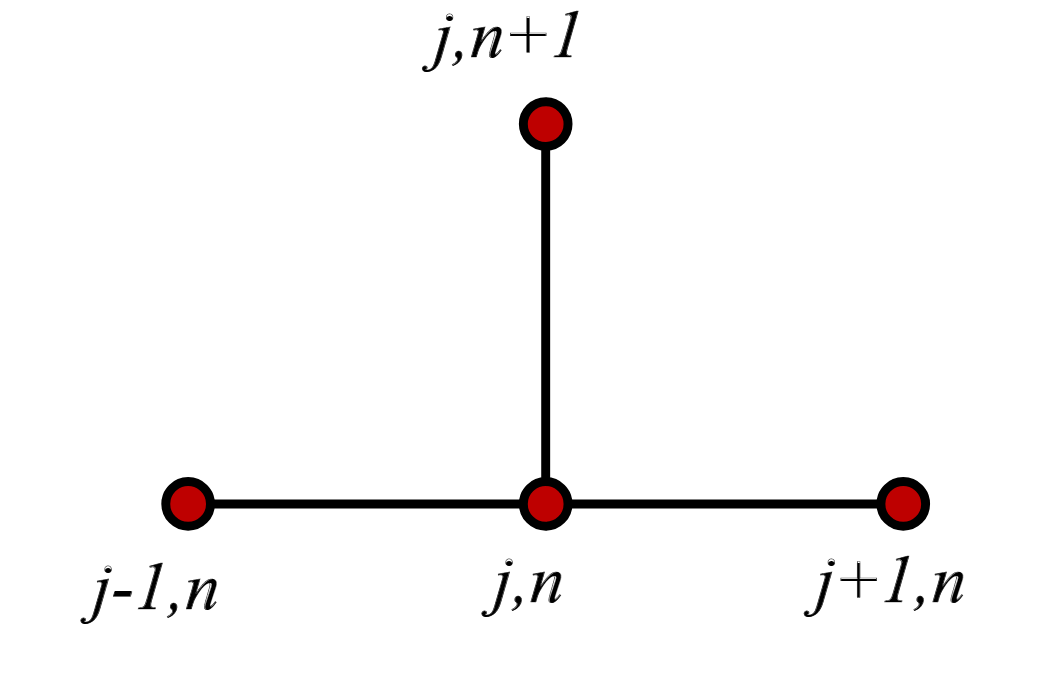
\includegraphics[scale=0.2]{Stencil.png}
    \caption{The Explicit Stencil which approximates the continuous time and space as a discrete mesh}
    \label{fig:stencil}
\end{figure}
In Sections 2 and 3 we formally introduce these schemes and analyse their consistency, stability and convergence. In Section 4 we verify our theoretical analysis through experimental methods, the consequences of which are discussed in Section 5.
\section{Finite Difference Approach}\label{sec:FDM}
    The Finite Difference method works, as stated in the introduction, by approximating the continuous space and time as a discrete grid of points. Thus the dependent variable $u(x_{i},t_{n})$ can be reformulated as $u_{i}^{n}$, where $i$ denotes a position in space and $n$ denotes a moment in time.
    \newline
    Since the explicit form of the method is used, $u_{i}^{n+1}$ is determined by some combination of $u_{i-1}^{n}$, $u_{i}^{n}$ and $u_{i+1}^{n}$, derived below.
	\subsection{Methodology}\label{sec:FDmethods}
	\begin{proof}[]
		We begin with (\ref{eq:fisher}),
		\begin{equation*}
		    \frac{\partial u}{\partial t} = \frac{\partial^2 u}{\partial x^2} + \rho u(1-u)
		\end{equation*}
		Using the Taylor Series expansion, we approximate the temporal derivative with a first order discretised approximation
		\begin{equation*}
		    u_{t}(x_{i},t_{n}) = \frac{u(x_{i},t_{n+1})-u(x_{i},t_{n})}{\Delta t} + O(\Delta t) = \frac{u_{i}^{n+1}-u_{i}^{n}}{\Delta t} + O(\Delta t)
		\end{equation*}
		Similarly, we approximate the second order spatial derivative with a second order discretised approximation
		\begin{equation*}
		\begin{split}
		    u_{xx}(x_{i},t_{n}) & = \frac{u(x_{i+1},t_{n})-2u(x_{i},t_{n})+u(x_{i-1},t_{n})}{\Delta x^2} + O(\Delta x^2) \\
		    & = \frac{u_{i+1}^{n}-2u_{i}^{n}+u_{i-1}^{n}}{\Delta x^2} + O(\Delta x^2)
		\end{split}
		\end{equation*}
		Dropping the truncation errors, we obtain
		\begin{equation}\label{eq:utFD}
		    u_{t}(x_{i},t_{n}) = \frac{u_{i}^{n+1}-u_{i}^{n}}{\Delta t}
		\end{equation}
		\begin{equation}\label{eq:uxxFD}
		    u_{xx}(x_{i},t_{n}) = \frac{u_{i+1}^{n}-2u_{i}^{n}+u_{i-1}^{n}}{\Delta x^2}
		\end{equation}
		Inserting equations (\ref{eq:utFD}) and (\ref{eq:uxxFD}) into equation (\ref{eq:fisher}), we arrive at
		\begin{equation}\label{eq:almostFiniteScheme}
		    \frac{u_{i}^{n+1}-u_{i}^{n}}{\Delta t} = \frac{u_{i+1}^{n}-2u_{i}^{n}+u_{i-1}^{n}}{\Delta x^2} + \rho u_{i}^{n}(1-u_{i}^{n})
		\end{equation}
		Which can be rearranged to arrive at our scheme
		\begin{equation}\label{eq:finiteScheme}
		    u_{i}^{n+1} = u_{i}^{n} + R(u_{i+1}^{n}-2u_{i}^{n}+u_{i-1}^{n}) + \rho \Delta t u_{i}^{n}(1-u_{i}^{n})
		\end{equation}
		where $R = \frac{\Delta t}{\Delta x^2}$
		
	\subsection{Analysis}\label{sec:FDanalysis}
	To prove the efficacy and usefulness of the approach, we prove consistency, stability (via von Neumann Stability Analysis) and convergence.
	\subsubsection{Consistency}
	To show consistency, we begin with (\ref{eq:almostFiniteScheme}), which of course is just a rearrangement of the scheme derived above.
	\begin{equation*}
		    \frac{u_{i}^{n+1}-u_{i}^{n}}{\Delta t} = \frac{u_{i+1}^{n}-2u_{i}^{n}+u_{i-1}^{n}}{\Delta x^2} + \rho u_{i}^{n}(1-u_{i}^{n})
	\end{equation*}
	Taking the limits to 0 of the step sizes $\Delta x$ and $\Delta t$
	\begin{equation*}
	\begin{split}
	    \lim_{\Delta x\to0,\Delta t\to0}\frac{u_{i}^{n+1}-u_{i}^{n}}{\Delta t} & = \lim_{\Delta x\to0,\Delta t\to0}\frac{u_{i+1}^{n}-2u_{i}^{n}+u_{i-1}^{n}}{\Delta x^2}\\ 
	    & + \lim_{\Delta x\to0,\Delta t\to0}\rho u_{i}^{n}(1-u_{i}^{n})
	\end{split}
	\end{equation*}
	Which, from the Taylor Series, recovers (\ref{eq:fisher}),
	\begin{equation*}
		    \frac{\partial u}{\partial t} = \frac{\partial^2 u}{\partial x^2} + \rho u(1-u)
		\end{equation*}
	\end{proof}
	\subsubsection{Stability}
	\begin{proof}[]
	Consider our scheme from (\ref{eq:finiteScheme}). 
	    \begin{equation*}
	        u_{i}^{n+1} = u_{i}^{n} + R(u_{i+1}^{n}-2u_{i}^{n}+u_{i-1}^{n}) + \rho \Delta t u_{i}^{n}(1-u_{i}^{n})
	    \end{equation*}
	    We assume an Ansatz in the form of a Fourier mode
        \begin{equation*}
        u_{i}^{n} = \xi^{n}e^{Iqi\Delta x}
        \end{equation*}
        where $q$ is a real spatial wave number of the Fourier series , $I = (-1)^{0.5}$ and $i$ and $n$ are the usual indices. We linearise the scheme by replacing the $u_{i}^{n}(1-u_{i}^{n})$ with $u_{i}^{n}(1-C)$, where $C$ is constant.
        \begin{equation*}
            u_{i}^{n+1} = u_{i}^{n} + R(u_{i+1}^{n}-2u_{i}^{n}+u_{i-1}^{n}) + \rho \Delta t u_{i}^{n}(1-C)
        \end{equation*}
	    Substituting this Ansatz into our numerical scheme, we arrive at
        \begin{equation*}
        \begin{split}
            \xi^{n+1}e^{Iqi\Delta x} &= \xi^{n}e^{Iqi\Delta x} + R\xi^{n}(e^{Iq(i+1)\Delta x} - 2e^{Iqi\Delta x}
              + e^{Iq(i-1)\Delta x}) \\ 
             & + \rho\Delta t\xi^{n}e^{Iqi\Delta x}(1 - C)
        \end{split}
         \end{equation*}
        Dividing through by $\xi^{n}e^{Iqi\Delta x }$ we get 
        \begin{equation*}
            \xi = 1 + R(e^{Iq\Delta x} - 2 + e^{-Iq\Delta x})+\rho\Delta t(1 - C))
        \end{equation*}
        \begin{equation*}
             \implies \xi = 1 + 2R(\frac{e^{Iq\Delta x} + e^{-Iq\Delta x}}{2} - 1) + \rho\Delta x(1  - C )
        \end{equation*}
        Now using Euler's formula and the double angle formula for $\cos(\theta)$ we get,
        \begin{equation*}
             \xi = 1 - 4R(\sin^{2}(\frac{q\Delta x}{2}) ) + \rho \Delta t (1 - C)
        \end{equation*}
	    for our scheme to be stable, we need  the amplification factor $-1<\xi<1$. The conditions we need for $\Delta x $ and $ \Delta t$ such that $-1<\xi<1$ holds is,
	    \begin{equation*}
	        -1 < 1 - 4R(\sin^{2}(\frac{q\Delta x}{2}) ) + \rho \Delta t (1 - C) < 1
	    \end{equation*}
	    Equivalently,
	    \begin{equation}\label{eq:doubleInequalityFD}
	        0 < 2 - 4R(\sin^{2}(\frac{q\Delta x}{2}) ) + \rho \Delta t (1 - C) < 2
	    \end{equation}
	    Now taking the RHS of equation (\ref{eq:doubleInequalityFD}) we have that 
	    \begin{equation*}
	        \implies 2 -4R(\sin^{2}(\frac{q \Delta x}{2})) + \rho\Delta t(1 - C) < 2
	    \end{equation*}
	    \begin{equation*}
	        \implies \rho \Delta t (1-C) < 4R\sin^{2}(\frac{q\Delta x}{2})
	    \end{equation*}
	     We note that $\max(\sin^{2}(\frac{q\Delta x}{2})) = 1$. Thus 
	     \begin{equation*}
	       \implies \rho\Delta t(1 - C) < 4R 
	     \end{equation*}
	     We choose $C=0$ in order to maximise $(1-u_{i}^{n})$ for $u_{i}^{n}>0$
	     \begin{equation*}
	         \rho\Delta t < 4R
	     \end{equation*}
	     \begin{equation*}
	         \implies R >\frac{\rho\Delta t}{4}
	     \end{equation*}
	     Now consider the LHS of equation (\ref{eq:doubleInequalityFD})
	     \begin{equation*}
	         -1 < 1 - 4R\sin^{2}(\frac{q\Delta x}{2}) + \rho\Delta t(1 -C)
	     \end{equation*}
	     Since $max(\sin^{2}(\frac{q\Delta x}{2})) = 1$ and $C = 0$, we obtain
	     \begin{equation*}
	      4R < 2 + \rho\Delta t
	     \end{equation*}
	     \begin{equation*}
	         \implies R< \frac{2 + \rho\Delta t}{4}
	     \end{equation*}
	     Thus the Finite Difference scheme is conditionally stable for $\frac{\rho \Delta t}{4} < R < \frac{2 + \rho\Delta t}{4}$. Expressed in terms of $\Delta x$ and $\Delta t$
	     \begin{equation}\label{eq:finiteDifferenceStability}
	         \frac{4 \Delta t}{2+\rho \Delta t} < \Delta x^2 < \frac{4}{\rho}
	     \end{equation}
	\end{proof}
	\subsubsection{Convergence}
	\begin{proof}[]
	    By the Lax Equivalence Theorem, the scheme is convergent.
	\end{proof}

\section{Non-Standard Finite Difference Approach}\label{sec:Alt}
    We now examine the Non-Standard Finite Difference approach, Introduced by R.E. Mickens. \cite{mickens}. 
	\subsection{Methodology}\label{sec:Altmethods}
		From \ref{eq:fisher} we have
		\begin{equation*}
		    \frac{\partial u}{\partial t} = \frac{\partial^2 u}{\partial x^2} + \rho u- \rho u^2
		\end{equation*}
		
		
		We know that a finite difference scheme is considered non-standard if the non-linear term $\rho u^2$ is replaced by a non-local discretisation \cite{anguelov}. 
		Using the non-local discretisation in \cite{mickens}, we obtain 

		\begin{equation}\label{eq:almostNonStandard}
		   \frac{u_i^{n+1} -u_i^{n} }{\Delta t} = \frac{u_{i+1}^n - 2u_i^n + u_{i-1}^n }{\Delta x^2}+\rho u_i^n-\rho (\frac{u_{i+1}^n + u_i^n + u_{i-1}^n}{3})u_i^{n+1}
		\end{equation}
		with $u^2$ being replaced by the non-local discretisation $(\frac{u_{i+1}^n + u_i^n + u_{i-1}^n}{3})u_i^{n+1}$.
		
		Solving for $u_i^{n+1}$ we get
        \begin{equation}\label{eq:nonStandardScheme}
		    u_i^{n+1} = \frac{R(u_{i+1}^n + u_{i-1}^n) + u_i^n(1+\rho \Delta t -2R)}{1+(\frac{\rho \Delta t}{3})(u_{i+1}^n + u_i^n + u_{i-1}^n)}
		\end{equation}
		where $R=\frac{\Delta t}{\Delta x^2}$. This gives us our non-standard finite difference scheme.
		
	\subsection{Analysis}\label{sec:Altanalysis}
    	As with the Finite Difference method, we prove consistency, stability (via von Neumann Stability Analysis) and convergence.
		\subsubsection{Consistency}
		\begin{proof}[]
    		From (\ref{eq:almostNonStandard}) we get
    		\begin{equation*}
    		   \frac{u_i^{n+1} -u_i^{n} }{\Delta t} = \frac{u_{i+1}^n - 2u_i^n + u_{i-1}^n }{\Delta x^2}+\rho u_i^n-\rho (\frac{u_{i+1}^n + u_i^n + u_{i-1}^n}{3})u_i^{n+1}
    		\end{equation*}
    		Applying limits,
            \begin{equation*}
            \begin{split}
                 \lim_{\Delta x, \Delta t\rightarrow 0}\frac{u_i^{n+1} -u_i^{n} }{\Delta t} & = \lim_{\Delta x, \Delta t\rightarrow 0}\frac{u_{i+1}^n - 2u_i^n + u_{i-1}^n }{\Delta x^2} + \lim_{\Delta x, \Delta t\rightarrow 0}\rho u_i^n \\
                 & - \lim_{\Delta x, \Delta t\rightarrow 0}\rho (\frac{u_{i+1}^n + u_i^n + u_{i-1}^n}{3})u_i^{n+1}
            \end{split}
    		\end{equation*}
    		which, from Taylor series, recovers (1),
    		\begin{equation*}
    		    \frac{\partial u}{\partial t} = \frac{\partial^2 u}{\partial x^2} + \rho u - \rho u^2
    		\end{equation*}
		\end{proof}
		\subsubsection{Stability}
		\begin{proof}[]
    		    
        Rewriting our scheme (\ref{eq:nonStandardScheme}), we obtain
        \begin{align*}
            u_i^{n+1}  + \frac{\rho \Delta t}{3}(u_{i+1}^n + u_i^n + u_{i-1}^n)u_i^{n+1} = R(u_{i+1}^{n}-2u_{i}^{n}+u_{i-1}^{n})  + \rho\Delta t u_i^n+ u_i^n
        \end{align*}
        We assume an Ansatz in the form of a Fourier mode
        \begin{equation*}
        u_{i}^{n} = \xi^{n}e^{Iqi\Delta x}
        \end{equation*}
        where $q$ is a real spatial wave number of the Fourier series , $I = (-1)^{0.5}$ and $i$ and $n$ are the usual indices. We linearise the scheme by replacing the term $\frac{\rho \Delta t}{3}(u_{i+1}^n + u_i^n + u_{i-1}^n)u_i^{n+1}$ with $\frac{\rho \Delta t}{3}(C)u_i^{n+1}$, where $C$ is a constant, and get
        \begin{align*}
            u_i^{n+1}  + C\frac{\rho \Delta t}{3}u_i^{n+1} = R(u_{i+1}^{n}-2u_{i}^{n}+u_{i-1}^{n})  + \rho\Delta t u_i^n+ u_i^n
        \end{align*}
        Substituting this Ansatz into our numerical scheme, we arrive at
        \begin{equation*}
        \begin{split}
            \xi^{n+1}e^{Iqi\Delta x} + C\frac{\rho \Delta t}{3}\xi^{n+1}e^{Iqi\Delta x} &= R\xi^{n}(e^{Iq(i+1)\Delta x} - 2e^{Iqi\Delta x}
              + e^{Iq(i-1)\Delta x}) \\
              &+ \rho \Delta t \xi^{n}e^{Iqi\Delta x} + \xi^{n}e^{Iqi\Delta x} 
        \end{split}
         \end{equation*}
        Dividing through by $\xi^{n}e^{Iqi\Delta x }$ we get
        \begin{equation*}
            \xi [1 + C\frac{\rho \Delta t}{3}] = R(e^{Iq\Delta x} - 2 + e^{-Iq\Delta x}) + \rho \Delta t + 1
        \end{equation*}

        \begin{equation*}
             \implies \xi [1 + C\frac{\rho \Delta t}{3}] = 2R(\frac{e^{Iq\Delta x} + e^{-Iq\Delta x}}{2} - 1) + \rho \Delta t + 1
        \end{equation*}
        Now using Euler's formula and the double angle formula for $\cos(\theta)$ we get,
        \begin{equation*}
            \xi [1 + C\frac{\rho \Delta t}{3}] = - 4R(\sin^{2}(\frac{q\Delta x}{2}) ) + \rho \Delta t + 1
        \end{equation*}
        \begin{equation*}
            \implies \xi  = \frac{ 1 - 4R(\sin^{2}(\frac{q\Delta x}{2}) ) + \rho \Delta t}{[1 + C\frac{\rho \Delta t}{3}]}
        \end{equation*}
	    For our scheme to be stable, we need  the amplification factor $-1<\xi<1$. The condition we need for $\Delta x $ and $ \Delta t$ such that $-1<\xi<1$ holds is,
	    \begin{equation}\label{eq:doubleInequalityNSFD}
	        -1 <  \frac{ 1 - 4R(\sin^{2}(\frac{q\Delta x}{2}) ) + \rho \Delta t}{[1 + C\frac{\rho \Delta t}{3}]} < 1
	    \end{equation}
		Now taking the RHS of equation (\ref{eq:doubleInequalityNSFD}) we have that 
	    \begin{equation*}
             1 - 4R(\sin^{2}(\frac{q\Delta x}{2}) ) + \rho \Delta t < 1 + C\frac{\rho \Delta t}{3}
	    \end{equation*}
	    We note that $\max(\sin^{2}(\frac{q\Delta x}{2})) = 1$. Thus 
	     \begin{equation*}
	       - 4R(\sin^{2}(\frac{q\Delta x}{2}) ) <  C\frac{\rho \Delta t}{3} - \rho \Delta t 
	     \end{equation*}
	     We choose $C=0$, then
	     \begin{equation*}
	         \rho\Delta t < 4R
	     \end{equation*}
	     \begin{equation*}
	         \implies R >\frac{\rho\Delta t}{4}
	     \end{equation*}
	     
	     Now consider the LHS of equation (\ref{eq:doubleInequalityNSFD})
	     \begin{equation*}
	        -1 <  \frac{ 1 - 4R(\sin^{2}(\frac{q\Delta x}{2}) ) + \rho \Delta t}{[1 + C\frac{\rho \Delta t}{3}]}
	     \end{equation*}
	     Since $max(\sin^{2}(\frac{q\Delta x}{2})) = 1$ and $C = 0$, we obtain
	     \begin{equation*}
	      4R < 2 + \rho\Delta t
	     \end{equation*}
	     \begin{equation*}
	         \implies R< \frac{2 + \rho\Delta t}{4}
	     \end{equation*}
	     Thus the Non-Standard Finite Difference scheme is conditionally stable for $\frac{\rho \Delta t}{4} < R < \frac{2 + \rho\Delta t}{4}$. Expressed in terms of $\Delta x$ and $\Delta t$
	     \begin{equation}\label{eq:finiteDifferenceStability}
	         \frac{4 \Delta t}{2+\rho \Delta t} < \Delta x^2 < \frac{4}{\rho}
	     \end{equation}
	     
    % 	  Consider the following scheme
    % 	    \begin{equation}
    % 	       u_{i}^{n+1} = \frac{R(u_{i+1}^{n})+(1+\rho\Delta t -2R)u_{i}^{n}}{1 + \rho\frac{\Delta t}{3}(u_{i+1}^{n} + u_{i}^{n} + u_{i+1}^{n})}
    % 	    \end{equation}
    % 	    Now consider the scheme in the following way
    % 	    \begin{equation}
    % 	        u_{i}^{n+1} = u_{i}^{n} + R(\delta _x)^2u_{i}^{n} + \Delta t\rho u_{i}^{n}(1-u_{i}^{n}) 
    % 	    \end{equation}
    % 	    where $(\delta _x)^2 = -4\sin^2{\frac{\Delta x q}{2}}$. The linear form of the above scheme is of the following way [4]
    % 	    \begin{equation}
    % 	        u_{i}^{n+1} = u_{i}^{n} R(\delta _x)^2u_{i}^{n} + \Delta t\rho u_{i}^{n}(1-constant)
    % 	    \end{equation}
    % 	    We assume an Ansatz in the form of a Fourier mode
    % 	    \begin{equation}
    % 	        u_{i}^{n} = \xi^{n}e^{Iqi\Delta x}
    % 	    \end{equation}
    % 	    substituting this Ansatz into our numerical scheme we get
    % 	    \begin{equation}
    % 	        \xi^{n+1}e^{Iqi\Delta x} = \xi^{n}e^{Iqi\Delta x} + R(\delta _x)^2\xi ^{n}e^{Iqi\Delta x} + \Delta t\rho\xi^{n}e^{Iqi\Delta x}(1- constant)
    % 	    \end{equation}
    % 	    Divide through by $\xi^{n}e^{Iqi\Delta x}$,we get
    % 	    \begin{equation}
    % 	        \xi = 1 + R(\delta _x)^2 + \Delta t\rho(1 - constant)
    % 	    \end{equation}
    % 	    \begin{equation}
    % 	        \implies \xi = 1 - 4R\sin^{2}(\frac{q\Delta x }{2}) + \Delta t\rho(1 - constant) 
    % 	    \end{equation}
    % 	    for our scheme to be stable, we need  the amplification factor $-1<\xi<1$. The conditions we need for $\Delta x $ and $ \Delta t$ so that $-1<\xi<1$ holds is,
    % 	    \begin{equation}
    % 	        -1 < 1 - 4Rsin^{2}(\frac{q\Delta x }{2}) + \Delta t\rho(1 - constant) < 1
    % 	    \end{equation}
    % 	    Now consider the RHS of (34)
    % 	    \begin{equation}
    % 	        1 - 4R\sin^{2}(\frac{q\Delta x }{2}) + \Delta t\rho(1 - constant) < 1
    % 	    \end{equation}
    % 	    \begin{equation*}
    % 	        \implies  \Delta t\rho(1 - constant) < 4R\sin^{2}(\frac{q\Delta x}{2}) 
    % 	    \end{equation*}
    % 	    since $\max[\sin^2{\frac{q\Delta x}{2}}] = 1$ and chose $constant = 0$. We get the following 
    % 	    \begin{equation}
    % 	        \frac{\Delta t \rho}{4} < R.
    % 	    \end{equation}
    % 	    Now consider LHS
    % 	    \begin{equation}
    % 	        -1 < 1 - 4R\sin^2{\frac{(q\Delta x)}{2}} + \Delta t \rho(1 - constant)
    % 	    \end{equation}
    % 	    \begin{equation}
    % 	        -2 < -4R\sin^{\frac{q\Delta x}{2}} +\Delta t \rho(1 - constant)
    % 	    \end{equation}
    % 	    \begin{equation}
    % 	        \implies 2 + \Delta t\rho(1-constant) > 4R\sin^2{(\frac{q\Delta x}{2})}
    % 	    \end{equation}
    % 	     since $\max[\sin^2{\frac{q\Delta x}{2}}] = 1$ and chose $constant = 0$. We get the following
    % 	     \begin{equation}
    % 	         2 + \Delta t\rho > 4R
    % 	     \end{equation}
    % 	     \begin{equation}
    % 	         \implies \frac{2+\Delta t\rho}{4} > R
    % 	     \end{equation}
    We note that this condition is identical to that imposed by the Finite Difference scheme.
    	\end{proof}
		\subsubsection{Convergence}
	    \begin{proof}[]
	        By the Lax Equivalence Theorem, the scheme is convergent.
    	\end{proof}
		
\section{Results}\label{sec:results}
	\subsection{Finite Difference Method}
	Comparing the Finite Difference scheme to the true solution, we obtained the following errors at $t=0.005$, using the initial condition of $u(x,0)=\frac{1}{(\exp{10\sqrt{\frac{10}{3}}x}+1)^2}$ and Dirichlet boundary conditions $u(-1, t) = 1$ and $u(1, t) = 0$, with $\rho =2000$, we get the following:
    	
    	\begin{table}[H]
            \begin{tabular}{|l|l|l|l|}
            \hline
            Experiment & $\Delta x$ & $\Delta t$   & $L_2$ Error \\ \hline
            1          & 0.05       & 0.00125      & 37.6239\\ \hline
            2          & 0.025      & 0.0003125    & 1.0009\\ \hline
            3          & 0.0125     & 0.000078125  & 0.2235\\ \hline
            4          & 0.00625    & 0.0000195313 & 0.0324\\ \hline
            \end{tabular}
        \end{table}
     Plotting the errors against the experiment number, we received the following results.
    \begin{figure}[H]
    \caption{$L_{2}$ Error vs. Experiment Number}
    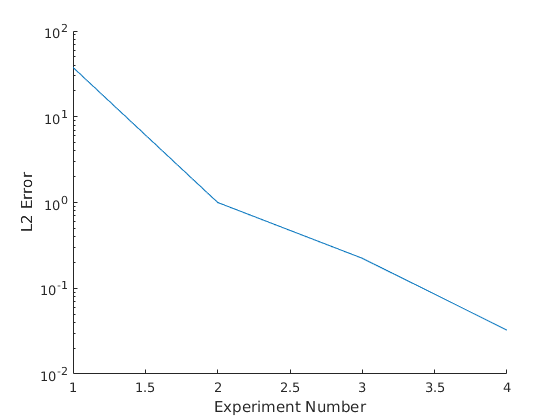
\includegraphics[scale=0.5]{FiniteDifferenceError.png}
    \end{figure}
    The huge error for experiment one is indicative of the numerical instability caused by the overly large step sizes. This instability is depicted in the mesh plot below.
    \begin{figure}[H]
    \caption{Numerical Instability in the Finite Difference Approach}
    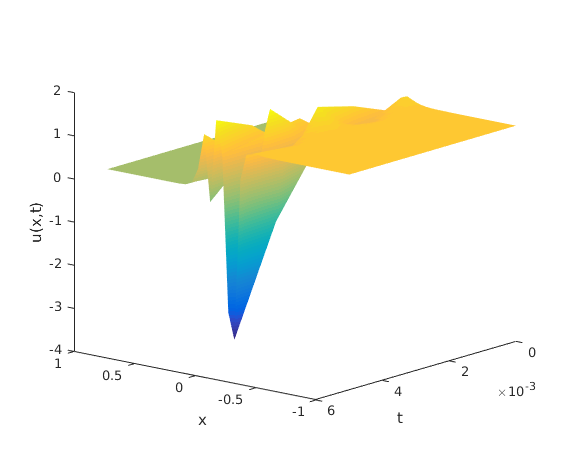
\includegraphics[scale=0.5]{Fisher_Dirichlet_NumericalInstability.png}
    \end{figure}
    This instability is expected, as the value for $\Delta x$ in experiment 1 does not satisfy the stability condition outlined in (\ref{eq:finiteDifferenceStability}).
    \newline
    Plotting a mesh plot of the scheme in the Dirichlet Boundary case, using the values $\Delta x = 0.00625$ and $\Delta t = 0.0000195313$ produces the following.
    \begin{figure}[H]
    \caption{Finite Difference Approximation with Dirichlet Boundaries}
    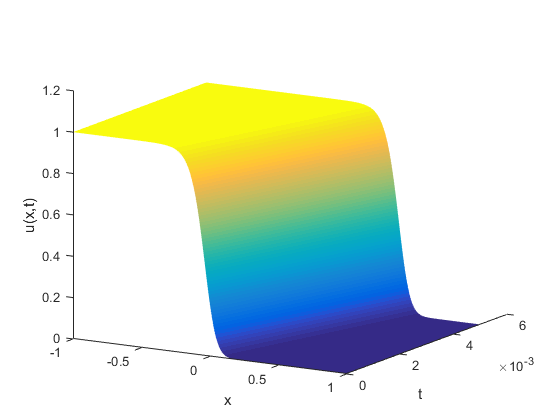
\includegraphics[scale=0.7]{Fisher_Dirichlet_FiniteDifference.png}
    \end{figure}
    The Neumann Boundary case, $u_{x}(-1,t) = 0$ and $u_{x}(1,t) = 0$, for the same values of $\Delta x$ and $\Delta t$ the plot as follows:
    \begin{figure}[H]
    \caption{Finite Difference Approximation with Neumann Boundaries}
    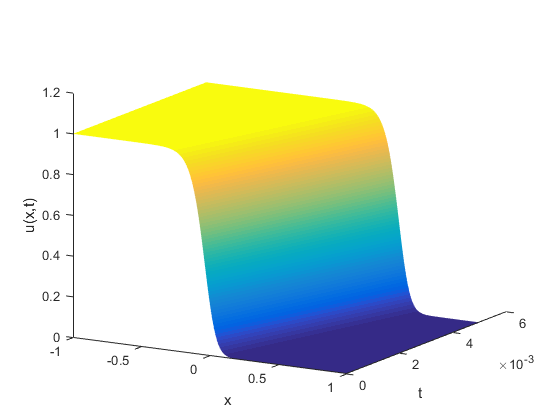
\includegraphics[scale=0.7]{Fisher_Neumann_FiniteDifference.png}
    \end{figure}
    \newpage
	\subsection{Non-Standard Finite Difference Method}
    	Comparing the Non-Standard Finite Difference scheme to the true solution, we obtained the following errors at $t=0.005$, using the initial condition of $u(x,0)=\frac{1}{(\exp{10\sqrt{\frac{10}{3}}x}+1)^2}$ and Dirichlet boundary conditions $u(-1, t) = 1$ and $u(1, t) = 0$, with $\rho =2000$, we get the following:
    	
    	\begin{table}[H]
            \begin{tabular}{|l|l|l|l|}
            \hline
            Experiment & $\Delta x$ & $\Delta t$   & $L_2$ Error \\ \hline
            1          & 0.05       & 0.00125      & 2.3075\\ \hline
            2          & 0.025      & 0.0003125    & 1.3537\\ \hline
            3          & 0.0125     & 0.000078125  & 0.3262\\ \hline
            4          & 0.00625    & 0.0000195313 & 0.0488\\ \hline
            \end{tabular}
        \end{table}
	
	Plotting the errors against the experiment number, we received the following results.
    \begin{figure}[H]
    \caption{$L_{2}$ Error vs. Experiment Number}
    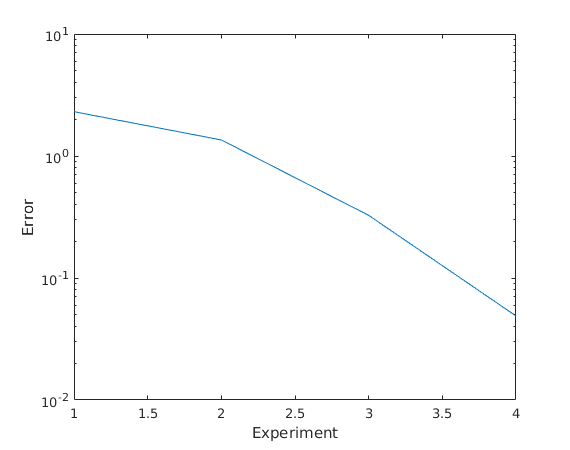
\includegraphics[scale=0.5]{ErrorNSFD.png}
    \end{figure}
	
    Plotting a mesh plot of the scheme in the Dirichlet Boundary case, using the values $\Delta x = 0.00625$ and $\Delta t = 0.0000195313$ produces the following.
    \begin{figure}[H]
    \caption{Non-Standard Finite Difference Approximation with Dirichlet Boundaries}
    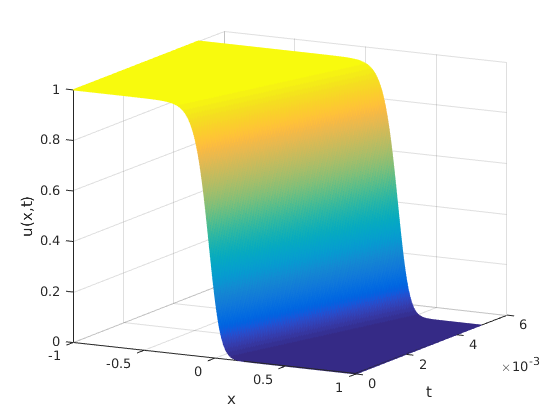
\includegraphics[scale=0.7]{Fisher_Dirichlet_NSFD.png}
    \end{figure}
	
	The Neumann Boundary case, $u_{x}(-1,t) = 0$ and $u_{x}(1,t) = 0$, for the same values of $\Delta x$ and $\Delta t$ the plot as follows:
    \begin{figure}[H]
    \caption{Non-Standard Finite Difference Approximation with Neumann Boundaries}
    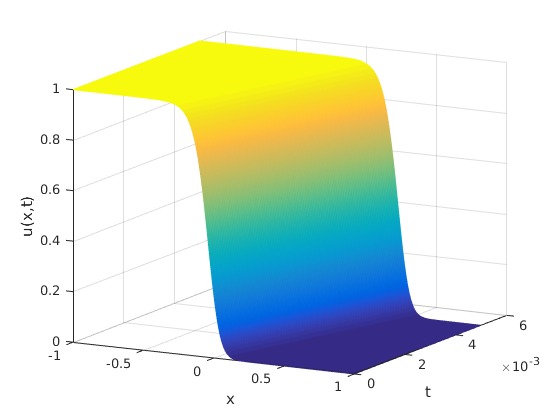
\includegraphics[scale=0.7]{Fisher_Nuemann_NSFD.png}
    \end{figure}
	
\section{Discussion}\label{sec:discussion}
    Both methods approximate the solution, a travelling wave front, quite well, numerical instabilities aside.
    \newline
    Plotting the errors from section 4.1 and 4.2 on a single graph, we obtain the following:
    \begin{figure}[H]
    \caption{$L_{2}$ Error vs. Experiment Number}
    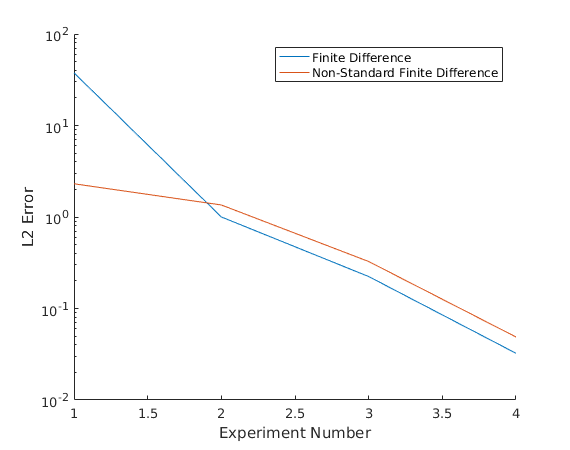
\includegraphics[scale=0.7]{ErrorComparison.png}
    \end{figure}
    Clearly, the Non-Standard Finite Difference approach vastly outperforms the Finite Difference approach in the first experiment, where the step sizes $\Delta x$ and $\Delta t$ are relatively large. However, from experiment 2 onward, where the step sizes are sufficiently small to ensure stability for both methods during the time interval, the Finite Difference approach approximates the solution slightly better than the Non-Standard Finite Difference approach. The fact that the two methods perform so similarly is not surprising, given that they differ only in their expression for $u^2$ and that they have identical conditions for stability, given our linearisations.
    \newline
    In terms of time complexity, both algorithms are $\mathcal{O}(TN)$, where $N$ is the number of spatial points and $T$ is the number of temporal points. Thus neither algorithm can be said to be better or worse with regards to computation. 
    \newpage
 \section{Conclusion}\label{sec:conclusion}
    Having analysed at length both the Finite Difference and Non-Standard Finite Difference approaches using both theoretical and experimental techniques, we conclude that, while both approaches are very similar, the Non-Standard Finite Difference method is more robust, coping better with overly large step sizes while performing admirably with small ones, at least in the case of the Fisher Equation. 
    \newline
    Although the Finite Difference method performs better than the Non-Standard Finite Difference method in this case, the fact that it succumbs to numerical instability more easily does not recommend it against the Non-Standard scheme. Furthermore, its performance hinges on small step sizes, therefore requiring many more points for the same interval. Depending on the size of the space and time intervals, such small step sizes may not be feasible.
    \newline
    Since the two methods perform so similarly, we suggest further research into their comparison. In particular, we suggest performing the experimental analysis for many more configurations of $\Delta x$ and $\Delta t$, in order to truly gauge their effect on the methods' efficacy. We further suggest that the robustness of each method be investigated over longer time intervals, where the effects of minor errors and instabilities become more pronounced. Finally, we suggest extending these methods to other equations, both within the Reaction-Diffusion class and beyond, in order to determine their performance across multiple equations.
    
\begin{thebibliography}{9}
    
\bibitem{mickens} 
    Mickens, Ronald E. Nonstandard finite difference schemes for reaction‐diffusion equations. \emph{Numerical Methods for Partial Differential Equations: An International Journal} 15.2 (1999): 201-214.

\bibitem{mickens2} 
Mickens, Ronald E. Applications of nonstandard finite difference schemes. \emph{World Scientific}, 2000.


\bibitem{anguelov} 
    Anguelov, R., P. Kama, and JM-S. Lubuma. On non-standard finite difference models of reaction–diffusion equations. \emph{Journal of computational and Applied Mathematics} 175.1 (2005): 11-29.

    
\bibitem{fisher}
    Fisher, R. The Wave of Advance of Advantageous Genes. \emph{Annals of Human Genetics}, June 1937.
\end{thebibliography}
\newpage
\appendix
\appendixpage

\section{Finite Difference Method Code}
\subsection{Dirichlet Case}
\lstinputlisting{Fisher_Dirichlet_FiniteDifference.m}
\subsection{Neumann Case}
\lstinputlisting{Fisher_Neumann_FiniteDifference.m}

\break
\section{Non-Standard Finite Difference Method Code}
\lstinputlisting{main_NSFD.m}
\subsection{Dirichlet Case}
\lstinputlisting{NSFD_Dirichlet.m}
\subsection{Neumann Case}
\lstinputlisting{NSFD_Neumann.m}

\end{document}